1\documentclass{beamer}
\usetheme{Frankfurt}

\usepackage{listings}

\newcommand{\todo}[1]{\alert{TODO #1}}

\title{Firewalls}
\subtitle{Lecture 5 \\ Computer Security DD2395}
\author[R. Guanciale]{
  Roberto Guanciale\\
  robertog@kth.se
}
\date{2015-11-12}
\begin{document}

\begin{frame}[plain]
  \titlepage
\end{frame}

\begin{frame}{Firewall/Iptables Lab}
  \begin{itemize}
  \item Preparation at home, fill out form in instructions 
  \item Lab at CSC, be there at start of lab slot 
  \item Lab exercise takes 4 hours
  \end{itemize}
\end{frame}

\begin{frame}{Seminar}
  \begin{itemize}
  \item 
  \end{itemize}
\end{frame}


\begin{frame}{Firewalls}
  \begin{itemize}
  \item What they do 
  \item Where to put them 
    \begin{itemize}
    \item On the network layers 
    \item On the network topology
    \end{itemize}
  \end{itemize}
\end{frame}

\begin{frame}{Bruce Schneier}
  
  \begin{quote}
Coal-powered trains had a large furnace in the 
engine room, along with a pile of coal. The 
engineer would shovel coal into the engine. 
This process created coal dust, which was 
highly flammable. Occasionally the coal dust 
would catch fire, causing an engine fire that 
sometimes spread into the passenger cars. 
Since dead passengers reduced revenue, train 
engines were built with iron walls right behind 
the engine compartment. This stopped fires 
from spreading into the passenger cars, but 
didn't protect the engineer between the coal pile 
and the furnace.
  \end{quote}
\end{frame}

% \begin{frame}{Network Security}
%   \begin{itemize}
%   \item Ross Anderson: 
%   \item System security 
%   \item Filtering 
%   \item Intrusion detection 
%   \item Cryptography, securing links 
%   \end{itemize}
% \end{frame}

\begin{frame}{Firewalls and Intrusion Prevention Systems}
  \begin{itemize}
  \item Individual: secure workstations and servers 
  \item Whole network: also use firewall as perimeter 
    defence 
    \begin{itemize}
    \item single choke point to impose security
    \item complement host-protection
    \item mitigate time-to-patch attack window
    \end{itemize}
  \item Firewall one of the ``intrusion prevention systems''
  \end{itemize}
\end{frame}

\begin{frame}{Principle of Complete Mediaton}
  \begin{itemize}
    \item It is required that all accesses to objects be checked 
to ensure that they are allowed.
  \end{itemize}
\end{frame}

\begin{frame}{Reference Monitor}
  \begin{itemize}
  \item In operating systems: 
    \begin{itemize}
    \item All requests are checked, only authorized go 
      through 
    \item Monitor itself is tamper-proof 
    \item And verifiable 
    \end{itemize}
  \end{itemize}
\end{frame}

\begin{frame}{Ingress and Egress filtering}
  \begin{itemize}
    \item Incoming, outgoing traffic
  \end{itemize}
\end{frame}

\begin{frame}[t]{Firewall (IPSs) Capabilities \& Limits}
  \begin{itemize}
  \item capabilities: 
    \begin{itemize}
    \item defines a single choke point 
    \item provides a location for monitoring security events 
    \item convenient platform for some Internet functions such as 
      NAT, usage monitoring, IPSEC VPNs 
    \end{itemize}
  \item limitations?
    \only<2>{
      \begin{itemize}
    \item cannot protect against attacks bypassing firewall 
    \item may not protect fully against internal threats 
    \item improperly secure wireless LAN 
    \item laptop, PDA, portable storage device infected outside 
    then used inside
    \item Stuxnet
      \begin{itemize}
        \item initially spread using USB flash memories
        \item exploits to infect other computers in the private
          networks that are not directly connected to the Internet
        \item infects project files belonging to Siemens control software
      \end{itemize}
    \end{itemize}
  }
  \end{itemize}
\end{frame}

\begin{frame}{Types of Firewalls}
  
  \begin{center}
    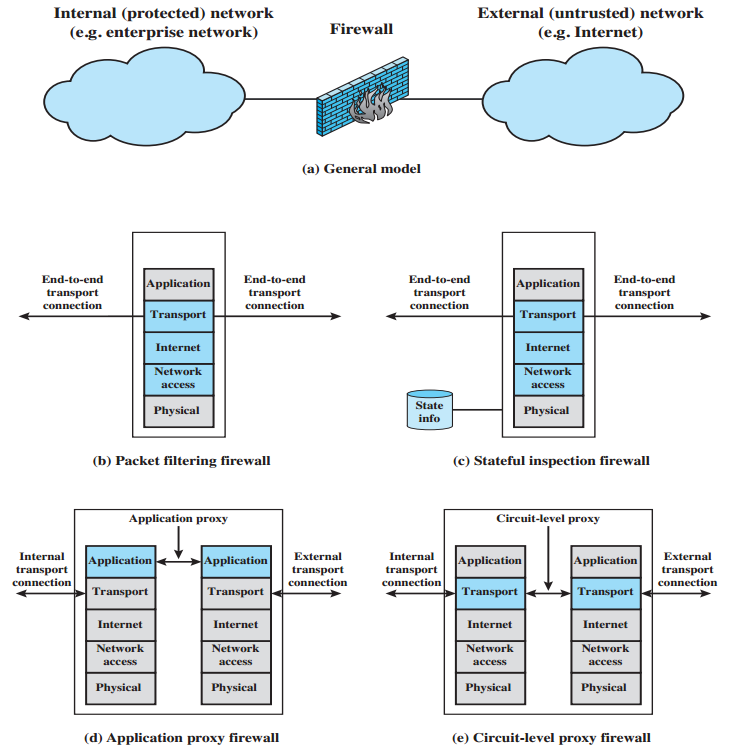
\includegraphics[width=0.6\linewidth]{firewall-type}
  \end{center}
\end{frame}

\begin{frame}{Packet Filtering Firewall}
  \begin{itemize}
  \item applies rules to packets in/out of firewall 
  \item based on information in packet header 
    \begin{itemize}
    \item src/dest IP addr \& port, IP protocol, interface 
    \end{itemize}
  \item typically a list of rules of matches on fields 
    \begin{itemize}
    \item if match rule says if forward or discard packet 
    \end{itemize}
  \item two default policies: 
    \begin{itemize}
    \item discard - prohibit unless expressly permitted 
      \begin{itemize}
      \item more conservative, controlled, visible to users 
      \end{itemize}
    \end{itemize}
    \begin{itemize}
    \item forward - permit unless expressly prohibited 
      \begin{itemize}
      \item easier to manage/use but less secure 
      \end{itemize}
    \end{itemize}
  \end{itemize}
\end{frame}

\begin{frame}{Packet Filter Rules}
  \begin{center}
    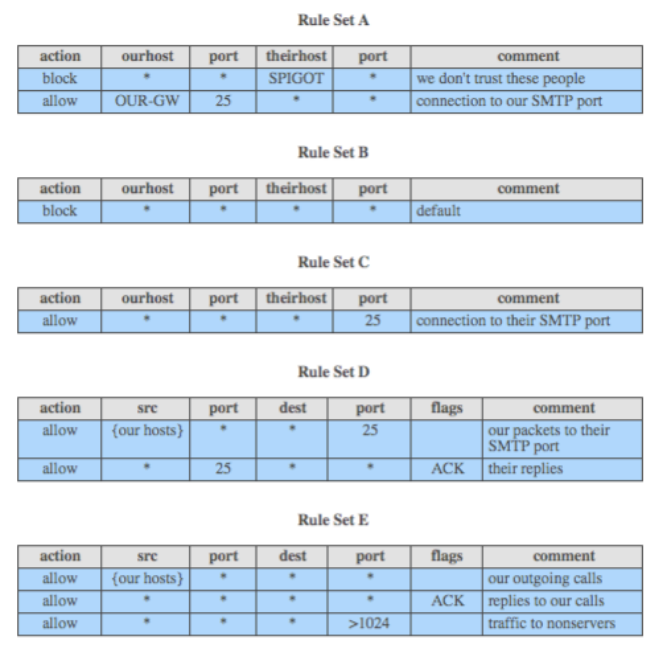
\includegraphics[width=0.6\linewidth]{filter-rules}
  \end{center}
\end{frame}

\begin{frame}{Packet Filter Weaknesses}
  \begin{itemize}
  \item weaknesses 
    \begin{itemize}
    \item cannot prevent attack on application bugs 
    \item limited logging functionality 
    \item do no support advanced user authentication 
    \item vulnerable to attacks on TCP/IP protocol bugs 
    \item improper configuration can lead to breaches
    \end{itemize}
  \end{itemize}
\end{frame}

\begin{frame}{Stateful Inspection Firewall}
  \begin{itemize}
  \item reviews packet header information but also keeps 
    info on TCP connections 
    \begin{itemize}
    \item typically have low, ``known'' port number for server 
    \item and high, dynamically assigned client port number
    \item simple packet filter must allow all return high port 
      numbered packets back in 
    \item stateful inspection packet firewall tightens rules for TCP 
      traffic using a directory of TCP connections 
    \item only allow incoming traffic to high-numbered ports for 
      packets matching an entry in this directory 
    \item may also track TCP seq numbers as well
    \end{itemize}
  \item can act as man in the middle
  \item Network address translation
  \end{itemize}
\end{frame}

\begin{frame}{Application-Level Gateway}
  \begin{itemize}
  \item acts as a relay of application-level traffic 
    \begin{itemize}
    \item user contacts gateway with remote host name 
    \item authenticates themselves 
    \item gateway contacts application on remote host and 
      relays TCP segments between server and user 
    \end{itemize}
  \item must have proxy code for each application 
    \begin{itemize}
    \item may restrict application features supported 
    \end{itemize}
  \item more secure than packet filters 
  \item but have higher overheads 
  \end{itemize}
\end{frame}

\begin{frame}{Circuit-Level Gateway}
  \begin{itemize}
  \item sets up two TCP connections, to an inside user 
    and to an outside host 
  \item relays TCP segments from one connection to 
    the other without examining contents 
    \begin{itemize}
    \item hence independent of application logic 
    \item just determines whether relay is permitted 
    \end{itemize}
  \item typically used when inside users trusted 
    \begin{itemize}
    \item may use application-level gateway inbound and 
      circuit-level gateway outbound 
    \item hence lower overheads
    \end{itemize}
  \end{itemize}
\end{frame}

\begin{frame}{Exchange and store ``filters''}
  \begin{itemize}
  \item 2009 - 2010 BredoLab botnet 30M hosts
  \item http://www.projecthoneypot.org/ Active stats (This Week)
  \begin{itemize}
      \item 3204 harvesters
      \item 285314 spam servers
      \item 7430 comment spammers
      \item 87457 dictionary attackers
      \item 344 rule breakers
    \end{itemize}
  \end{itemize}
\end{frame}

\begin{frame}{Bloom filter}
  \begin{itemize}
  \item Space-efficient probabilistic data structure for set membership
  \item False positive matches are possible
  \item False negatives are not
    \[
      x \not \in BF(S) \Rightarrow x \not \in S
    \]
  \item  A Bloom filter with $1\%$ error can be created using
    $\sim$ 9.6 bits per element
  \end{itemize}
\end{frame}

\begin{frame}[t]{Bloom filter}
  \begin{itemize}
  \item $m$-bit array
  \item $k$ hash functions $f_k : S \rightarrow [0, m-1]$
  \item $f_k$ independent functions with a uniform random distribution
  \item example: $m = 16$, $k=2$, $f_1(ip) = (ip.1+ip.3) \% m$,
    $f_2(ip) = (ip.2+ip.4) \% m$
  \end{itemize}
  \only<2> {
  $B = New() : for\  i \in [0, m-1]. B[i] := 0$\\
  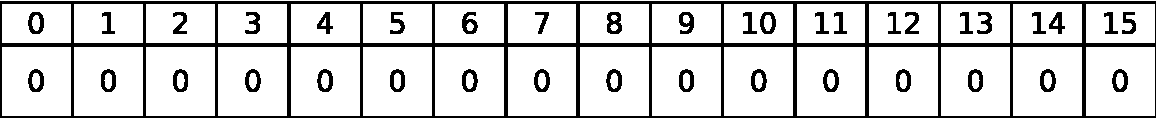
\includegraphics[width=0.8\linewidth]{bloom0}
  }
  \only<3-4> {
  $B = Add(B, x): for\ j \in [1,k], B[f_k(x)] := 1$\\
  }
  \only<3> {
  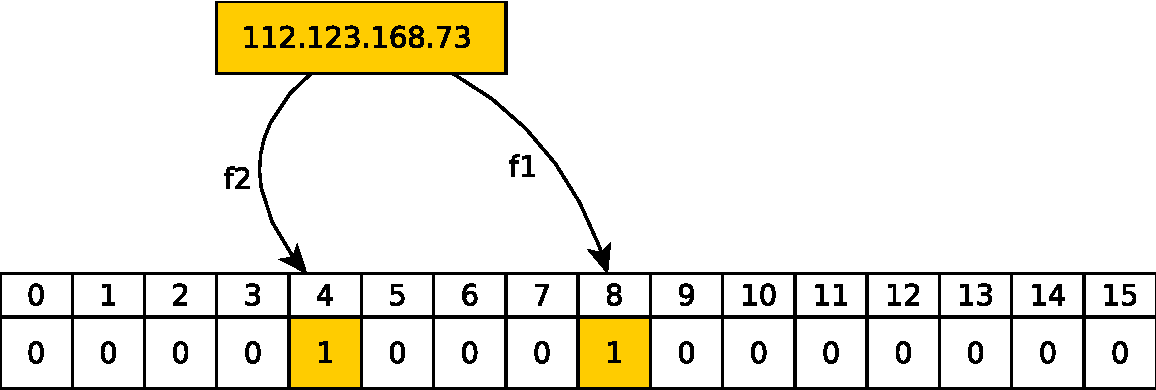
\includegraphics[width=0.8\linewidth]{bloom1}
  }
  \only<4> {
  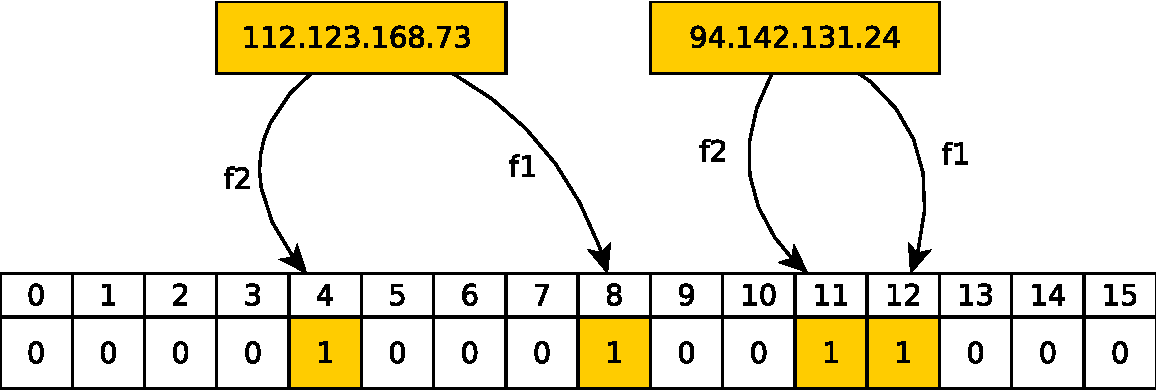
\includegraphics[width=0.8\linewidth]{bloom2}
  }
  \only<5> {
  $Query(B, x): \prod_{j \in [1,k]} B[f_k(x)] = 1$\\
  }
  \only<6> {
  Lossless union\\
  $B = B_1 \cup B_2: for\ i \in [0,m-1], B[i] = B_1[i] \vee B_2[i]$\\
  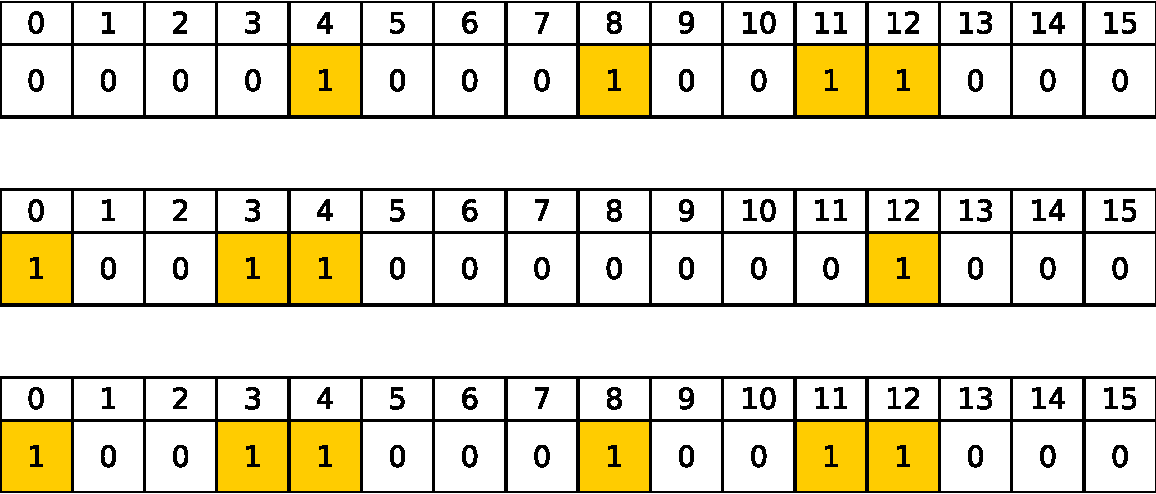
\includegraphics[width=0.8\linewidth]{bloom3}
  }
  \only<7> {
  Lossy intersection\\
  $B = B_1 \cap B_2: for\ i \in [0,m-1], B[i] = B_1[i] \wedge B_2[i]$\\
  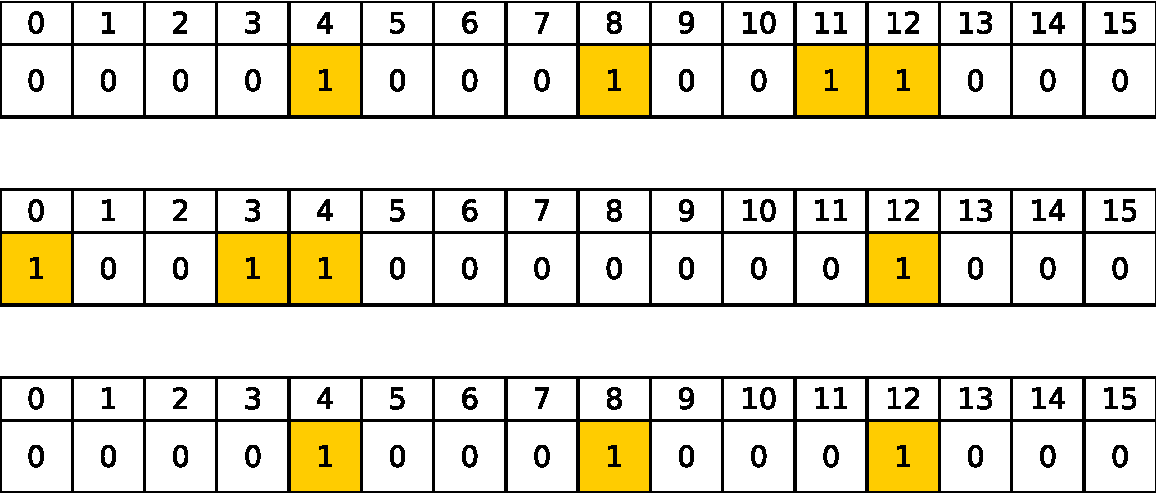
\includegraphics[width=0.8\linewidth]{bloom4}
  }
\end{frame}


\begin{frame}{Firewall Basing}
  \begin{itemize}
  \item several options for locating firewall: 
  \item bastion host 
  \item individual host-based firewall 
  \item personal firewall
  \end{itemize}
\end{frame}

\begin{frame}{Bastion Hosts}
  \begin{itemize}
  \item critical strongpoint in network 
  \item hosts application/circuit-level gateways 
  \item common characteristics: 
    \begin{itemize}
    \item runs secure O/S, only essential services 
    \item may require user auth to access proxy or host 
    \item each proxy can restrict features, hosts accessed 
    \item each proxy small, simple, checked for security 
    \item each proxy is independent, non-privileged 
    \item limited disk use, hence read-only code 
    \end{itemize}
  \end{itemize}
\end{frame}

\begin{frame}{Host-Based Firewalls}
  \begin{itemize}
  \item used to secure individual host 
  \item available in/add-on for many O/S 
  \item filter packet flows 
  \item often used on servers 
  \item advantages: 
    \begin{itemize}
    \item taylored filter rules for specific host needs 
    \item protection from both internal / external attacks 
    \item additional layer of protection to org firewall 
    \end{itemize}
  \end{itemize}
\end{frame}

\begin{frame}{Personal Firewall}
  \begin{itemize}
  \item controls traffic flow to/from PC/workstation 
  \item for both home or corporate use 
  \item may be software module on PC 
  \item or in home cable/DSL router/gateway 
  \item typically much less complex 
  \item primary role to deny unauthorized access 
  \item may also monitor outgoing traffic to detect/block 
    worm/malware activity
  \end{itemize}
\end{frame}

\begin{frame}{Firewall Topologies}
  \begin{itemize}
  \item host-resident firewall 
  \item screening router: packet filtering 
  \item single bastion inline between routers 
  \item single bastion T, with DMZ 
  \item double bastion inline: DMZ between bastions 
  \item double bastion T 
  \item distributed firewall configuration
  \end{itemize}
\end{frame}

\begin{frame}{Firewall Locations}
  \begin{columns}[c]
    \column{0.4\linewidth}
    \only<2> {
    \begin{itemize}
    \item advantages?
    \item disadvantages?
    \end{itemize}
    }
    \column{0.5\linewidth}
    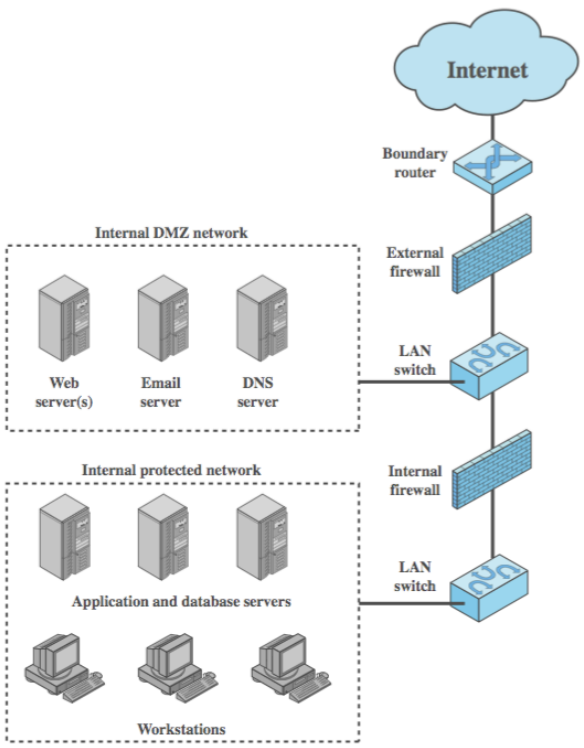
\includegraphics[width=1\linewidth]{firewall-location}
  \end{columns}
\end{frame}

\begin{frame}{Virtual Private Networks}
  \begin{center}
    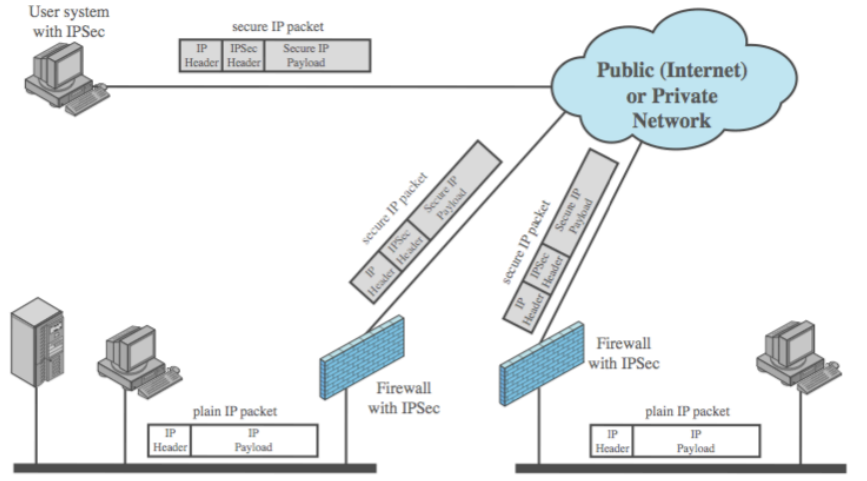
\includegraphics[width=1\linewidth]{vpn}
  \end{center}
\end{frame}

\begin{frame}{Distributed Firewalls}
  \begin{center}
    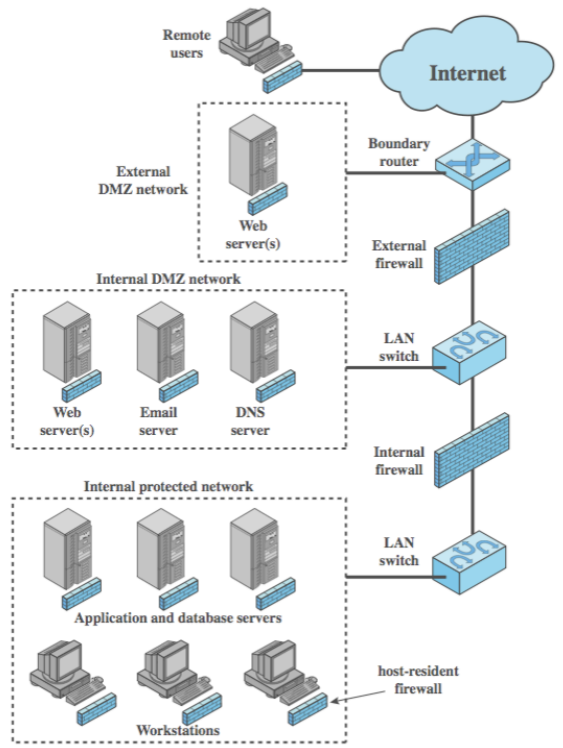
\includegraphics[width=0.5\linewidth]{distributed-firewalls}
  \end{center}
\end{frame}

\begin{frame}{Intrusion Prevention Systems (IPS)}
  \begin{itemize}
  \item recent addition to security products which 
    \begin{itemize}
    \item inline net/host-based IDS that can block traffic 
    \item functional addition to firewall that adds IDS 
      capabilities 
    \end{itemize}
  \item can block traffic like a firewall 
  \item using IDS algorithms 
  \item may be network or host based
  \end{itemize}
\end{frame}

\begin{frame}{Host-Based IPS}
  \begin{itemize}
  \item identifies attacks using both: 
    \begin{itemize}
    \item signature techniques 
      \begin{itemize}
      \item malicious application packets 
      \end{itemize}
    \item anomaly detection techniques 
      \begin{itemize}
      \item behavior patterns that indicate malware 
      \end{itemize}
    \end{itemize}
  \item can be tailored to the specific platform 
    \begin{itemize}
    \item e.g. general purpose, web/database server specific 
    \end{itemize}
  \item can also sandbox applets to monitor behavior 
  \item may give desktop file, registry, I/O protection
  \end{itemize}
\end{frame}

\begin{frame}{Network-Based IPS}
  \begin{itemize}
  \item inline NIDS that can discard packets or 
    terminate TCP connections 
  \item uses signature and anomaly detection 
  \item may provide flow data protection 
    \begin{itemize}
    \item monitoring full application flow content 
    \end{itemize}
  \item can identify malicious packets using: 
    \begin{itemize}
    \item pattern matching, stateful matching, protocol 
      anomaly, traffic anomaly, statistical anomaly 
    \end{itemize}
  \item cf. SNORT inline can drop/modify packets
  \end{itemize}
\end{frame}

\begin{frame}{An example: SMTP}
  \begin{itemize}
  \item TCP/IP vulnerabilities
    \begin{itemize}
    \item SYN flood/spoofing (packet filtering)
    \item external attacker using src port 25 (stateful inspection)
    \end{itemize}
  \item SMTP vulnerabilities
    \begin{itemize}
    \item sendmail buffer overflow (SE-Linux)
    \end{itemize}
  \item Mime vulnerabilities
    \begin{itemize}
    \item PNG buffer overflow (SMTP IPS/antivirus)
    \end{itemize}
  \item User vulnerabilities
    \begin{itemize}
    \item Phishing‎ (Train users/SMTP IPS/antispam)
    \end{itemize}
  \end{itemize}
\end{frame}

\begin{frame}{Antispam: naive Bayes classifier}
  \begin{itemize}
  \item probabilistic classifier based on applying Bayes' theorem
  \item assumes with strong (naive) independence assumption
  \item still effective
  \end{itemize}
\end{frame}

\begin{frame}{Antispam: naive Bayes classifier}
  \begin{itemize}
  \item \alert{Really naive assumptions}
  \item let $C$ be a class random variable: $C \in \{spam,ok\}$
  \item let $F_i$ be a feature random variable:
    \begin{itemize}
      \item $F_i \in \{true,false\}$  if the mail contains the word
        ``lottery''
      \item $F_i \in \{true,false\}$  if the mail sender is ``yahoo.com''
      \item $F_i \in \{0 \dots 24\}$  mail delivery hour
    \end{itemize}
  \item compute $P(C|F_1 \dots F_n)$
  \item if $P(C=spam|F_1 \dots F_n) > P(C=ok|F_1 \dots F_n)$ tag the email
  \end{itemize}
\end{frame}

\begin{frame}{Antispam: naive Bayes classifier}
  \begin{itemize}
    \only<1> {
  \item compute $P(C|F_1 \dots F_n)$
  \item Bayes' theorem
    \[
    P(C|F_1 \dots F_n) =
    \frac
    {P(C) P(F_1 \dots F_n | C) }
    {P(F_1 \dots F_n)}
    \]
  \item let $Z = P(F_1 \dots F_n)$, $Z$ does not depend on $C$
    \[
    P(C|F_1 \dots F_n) =
    \frac
    {P(C) P(F_1 \dots F_n | C) }
    {Z}
    \]
  }
  \item by Chain rule: $P(X_1 \dots X_n) = \prod{P(X_i | X_1 \dots X_{i-1})}$
    \[
    P(C|F_1 \dots F_n) =
    \frac
    {P(C) 
     \prod{P(F_i| (C,  F_1, \dots, F_{i-1})}
    }
    {Z}
    \]
  \item<2-> independence hypotheses $P(F_i| (C,  F_1, \dots, F_{i-1})
    = P(F_i| C)$
    \[
    P(C|F_1 \dots F_n) =
    \frac
    {P(C) 
     \prod{P(F_i| C)}
    }
    {Z}
    \]
  \end{itemize}
\end{frame}

\begin{frame}{Summary}
  \begin{itemize}
  \item introduced need for \& purpose of firewalls 
  \item types of firewalls 
    \begin{itemize}
    \item packet filter, stateful inspection, application and 
      circuit gateways 
    \end{itemize}
  \item firewall hosting, locations, topologies 
  \item intrusion prevention systems
  \end{itemize}
\end{frame}




















\end{document}




%%% Local Variables: 
%%% mode: latex
%%% TeX-master: t
%%% End: 
